\chapter{Variational method}
\label{ch:cl-var}

The MCMC method in the previous chapter is widely used to compute various observables of many-body systems. However, a limitation is that it is agnostic of the partition function $Z$ in \cref{eq:boltzmann}, therefore it cannot compute quantities that require $Z$ or the normalized probability $p_\text{B}(\vs)$, including the free energy and the entropy. Variants of MCMC have been proposed to compute $Z$, such as the Wang--Landau algorithm~\cite{wang2001efficient, landau2021guide5}. However, they also involve other issues such as the discretization of the energy histogram~\cite{belardinelli2007wang}, which limit their use in practical computations.

A different approach is to track the probability distribution in the framework of variational approximation and statistical inference~\cite{jordan1999introduction, mackay2003information}, which also has deep roots in statistical physics, traced back to mean-field theories~\cite{chaikin1995principles4, zdeborova2016statistical}. We define a trial distribution $q(\vs)$, or the ``ansatz'' in the context of statistical physics, to approximate the target distribution $p(\vs)$. The form of the ansatz is chosen so that the normalized probability $q(\vs)$ can be efficiently computed given a configuration $\vs$, and the distribution can be easier to sample from than $p(\vs)$, or even be analytically summed over in \cref{eq:cl-obs}. Some choices of the ansatz for variational inference will be discussed in \cref{sec:nmf}.

\section{Variational free energy}

To make a good approximation, we want the ansatz $q(\vs)$ to be as close to the target $p(\vs)$ as possible. A natural metric of the distance between two distributions is the Kullback--Leibler (KL) divergence~\cite{kullback1951information}:
\begin{equation}
D_\text{KL}(q \mid\mid p) = \sum_\vs q(\vs) \ln \frac{q(\vs)}{p(\vs)}.
\end{equation}
When $p(\vs)$ is the Boltzmann distribution, we have
\begin{align}
D_\text{KL}(q \mid\mid p_\text{B}) &= \sum_\vs q(\vs) \left( \ln q(\vs) - \ln \frac{\rme^{-\beta H(\vs)}}{Z} \right) \label{eq:kl} \\
&= \beta (F_q - F), \label{eq:kl-fq}
\end{align}
where $F = -\frac{1}{\beta} \ln Z$ is the true free energy, and we define the variational free energy
\begin{equation}
F_q = \sum_\vs q(\vs) F_\text{loc}(\vs),
\label{eq:fq}
\end{equation}
and the local free energy
\begin{equation}
F_\text{loc}(\vs) = \frac{1}{\beta} \ln q(\vs) + H(\vs).
\label{eq:fq-loc}
\end{equation}

Similar to how we have approximated \cref{eq:cl-obs} by \cref{eq:monte-carlo}, the variational free energy in \cref{eq:fq} is also a weighted sum over the distribution $q(\vs)$ with exponentially many terms, and we can estimate it by Monte Carlo sampling:
\begin{equation}
\bbE_\text{MC}[F_q] = \frac{1}{M} \sum_{i = 1}^M F_\text{loc}\left( \vs^{(i)} \right), \quad
\vs^{(i)} \sim q.
\label{eq:fq-monte-carlo}
\end{equation}
This method has close resemblance to the variational Monte Carlo (VMC) method for quantum systems, which we will discuss in the next part, although the term VMC is rarely used in the context of classical systems. It is worth noting that variational inference requires one to evaluate the normalized probability $q(\vs)$, in contrast to MCMC in the previous chapter where the normalization constant cancels out in the derivation of the Markov chain, as in \cref{eq:metropolis}. Therefore, it is important to choose an ansatz $q(\vs)$ whose probability is tractable.

\section{Minimization of variational free energy}

The ansatz $q(\vs)$ is usually controlled by some parameters $\theta$, which allows us to minimize the KL divergence by varying $\theta$. In \cref{eq:kl-fq}, the term $F$ is independent of $\theta$, so we only need to minimize $F_q$. As the KL divergence is non-negative, the lower bond of $F_q$ among all possible ansatzes is exactly the true free energy $F$, which is desired to compute in many cases. This property is known as the Bogolubov inequality~\cite{bogolubov1966model}. A common practice is to minimize $\beta F_q$ rather than $F_q$ itself, which avoids the singularity of $\frac{1}{\beta}$ in \cref{eq:fq} when $\beta \to 0$.

\subsection{Gradient descent optimizers}
\label{sec:gd}

As $F_q$ is generally a multivariate nonlinear function of $\theta$, its optimization is usually performed by gradient descent (GD)-based algorithms~\cite{curry1944method}. In the naive setting of GD, in each optimization step $t$ we update $\theta$ by
\begin{equation}
\theta_{t + 1} \gets \theta_t - \gamma \left. \nabla F_q \right|_{\theta = \theta_t},
\label{eq:gd}
\end{equation}
where $\nabla F_q = \frac{\partial F_q}{\partial \theta}$ is the gradient vector of the target function, and $\gamma$ is a small positive number called the learning rate. A common challenge in GD is to choose an appropriate magnitude of $\gamma$, such that the optimization is neither unstable nor too slow to converge~\cite{boyd2004convex}. Another challenge is to converge to the global minimum of the target function, rather than to be trapped by local minima and saddle points. It is particularly important in physical problems to find the global minimum accurately. In contrast to typical machine learning problems, such as computer vision, where one only seeks a ``good-looking'' solution that simulates the inaccurate nature of human vision, in physics there is great interest in obtaining quantitative properties to high accuracies. It is even more crucial to identify qualitative properties about the global minimum, such as symmetries of the ground state. This demand poses unique challenges to the optimization algorithms we use~\cite{chen2023efficient, michaud2023precision}.

When estimating the gradient in \cref{eq:gd}, we usually generate a set of random samples $\{\vs^{(1)}, \vs^{(2)}, \ldots, \vs^{(M)}\}$ in each sampling step, rather than sum over the exponentially large space of configurations. This practice is known as the stochastic gradient descent (SGD)~\cite{robbins1951stochastic, bottou1998online}, and the sample size $M$ is also known as the ``batch'' size in machine learning. In the continuous-time limit, SGD is equivalent to exact gradient flow with an additional Brownian noise~\cite{hu2017diffusion}, and the variance of the noise scales by $O\left( \frac{1}{M} \right)$. This Brownian motion is also equivalent to a simulated annealing, whose equilibrium distribution is a Boltzmann distribution\footnote{Not to be confused with the physical Boltzmann distribution in the space of the configurations $\vs$.} in the space of the parameter $\theta$. In other words, this noise helps the optimizer escape from local minima and saddle points, given an appropriate ratio of the learning rate to the batch size, which explains the successful application of SGD in various non-convex problems.

Many advanced variants of SGD have been proposed in the recent trend of machine learning~\cite{kashyap2022survey}. In particular, the Adam optimizer~\cite{kingma2015adam} has become the most popular among them. It estimates the appropriate learning rate for each parameter by the second moment\footnote{It is the second moment of the norms of each gradient components in the case of complex-valued gradients.} of the gradient, and uses the first moment to improve convergence, which largely reduces manual labor to tune the learning rate. Numerous experiments have demonstrated its broad applicability to machine learning problems, although its convergence properties are still debatable in physical problems that require high accuracy.

\subsection{Second-order optimizers}
\label{sec:ngd}

We refer to GD as a first-order optimizer\footnote{Not to be confused with the order of the convergence speed, which is related to the order in the definition of the optimizer, but not always equivalent.}, because it approximates the target function with only the first-order term in the Taylor expansion, which is the gradient. There are also various second-order optimizers that approximate the target function with a quadratic function, and utilize information about the Hessian matrix to precondition the gradient, i.e., to modify the direction and the magnitude of the gradient in order to reduce the condition number of the optimization problem and accelerate the convergence. The second-order optimizers date back to the Newton's method, which updates $\theta$ by
\begin{equation}
\theta_{t + 1} \gets \theta_t - \gamma \left. \mH^{-1} \nabla F_q \right|_{\theta = \theta_t},
\label{eq:newton}
\end{equation}
where $\mH$ is the Hessian matrix of the target function defined by $H_{i j} = \frac{\partial^2 F_q}{\partial \theta_i \partial \theta_j}$. In this case, the learning rate $\gamma$ can be close to $1$ if the target function is close to the quadratic approximation. However, this method can easily become unstable with highly nonlinear target functions, and an interpolation between the first- and the second-order updates is required to enhance stability, such as the Levenberg--Marquardt algorithm~\cite{levenberg1944method}. Moreover, directly storing $\mH$ requires $O(n_\text{p}^2)$ space, where $n_\text{p}$ is the number of parameters, and directly inverting it requires $O(n_\text{p}^3)$ computation, both of which are impractical with large numbers of parameters in neural networks. Therefore, modern methods approximate $\mH^{-1}$ with low-rank updates and line searches, such as the conjugate gradient method~\cite{fletcher1964function} and the limited-memory Broyden--Fletcher--Goldfarb--Shanno (L-BFGS) algorithm~\cite{liu1989limited}. Even with these improvements, the use of second-order optimizers is still hardly practical in large-scale machine learning problems, let alone higher-order ones.

When the target function is a KL divergence, a special technique is to replace $\mH$ in \cref{eq:newton} by the Fisher information matrix
\begin{equation}
\mS = \sum_\vs q(\vs) \nabla \ln q(\vs) \left( \nabla \ln q(\vs) \right)^\transpose.
\label{eq:fim}
\end{equation}
While in principle the gradient can be preconditioned by the inverse of any positive definite matrix, the Fisher information matrix is particularly useful, because it is a natural metric in the function space where the KL divergence measures the distance~\cite{martens2020new}. This technique is known as natural gradient descent (NGD)~\cite{amari1998natural}, and has led to another line of research to approximate it, such as the Kronecker factorization (K-FAC)~\cite{martens2015optimizing} and online approximations~\cite{roux2007topmoumoute, ollivier2017true}. We will give more discussion on NGD in the context of quantum problems in \cref{sec:sr}, where first-order optimizers produce unsatisfactory results and NGD is considered necessary.

\section{Gradient estimator}

The gradient $\nabla F_q$ in \cref{eq:gd} is derived by automatic differentiation (AD)~\cite{baydin2018automatic} in modern software\footnote{Specifically, the technique to derive the gradient of a scalar target function w.r.t.\ many parameters is named backpropagation, or reverse mode AD.}, which can be more accurate and efficient than traditional methods of finite difference and more prone to errors than manually deriving and implementing the gradient. Care should be taken that \cref{eq:fq} involves the distribution $q(\vs)$, which is a function of $\theta$, but this term no longer exists after replacing \cref{eq:fq} by \cref{eq:fq-monte-carlo}, and we cannot take the gradient of this term in the usual way after sampling the configurations in \cref{eq:fq-monte-carlo}. Therefore, we rewrite the gradient of \cref{eq:fq} as
\begin{align}
\frac{\partial F_q}{\partial \theta}
&= \sum_\vs \left( \frac{\partial q(\vs)}{\partial \theta} F_\text{loc}(\vs) + q(\vs) \frac{\partial F_\text{loc}(\vs)}{\partial \theta} \right) \\
&= \sum_\vs \left( q(\vs) \frac{\partial \ln q(\vs)}{\partial \theta} F_\text{loc}(\vs) + q(\vs) \frac{1}{\beta} \frac{\partial \ln q(\vs)}{\partial \theta} \right).
\label{eq:fq-grad-2-terms}
\end{align}
The second term of \cref{eq:fq-grad-2-terms} becomes
\begin{align}
&\phantom{{}={}}\frac{1}{\beta} \sum_\vs q(\vs) \frac{\partial \ln q(\vs)}{\partial \theta} \\
&= \frac{1}{\beta} \sum_\vs \frac{\partial q(\vs)}{\partial \theta} \\
&= \frac{1}{\beta} \frac{\partial}{\partial \theta} \sum_\vs q(\vs).
\end{align}
As we have the normalization $\sum_\vs q(\vs) = 1$, this term is always zero. The remaining first term of \cref{eq:fq-grad-2-terms} can be again estimated by Monte Carlo sampling:
\begin{equation}
\bbE_\text{MC}\left[ \frac{\partial F_q}{\partial \theta} \right]
= \frac{1}{M} \sum_{i = 1}^M F_\text{loc}\left( \vs^{(i)} \right) \frac{\partial \ln q\left( \vs^{(i)} \right)}{\partial \theta}, \quad
\vs^{(i)} \sim q.
\label{eq:fq-grad}
\end{equation}
This method is called the REINFORCE gradient~\cite{williams1992simple} or the policy gradient~\cite{sutton1999policy} in the context of machine learning, and the gradient of the log-probability $\frac{\partial \ln q(\vs)}{\partial \theta}$ is called the score function~\cite{fisher1935detection, hyvarinen2005estimation, mohamed2020monte}. This kind of differentiation through discrete variables and stochastic sampling of distributions is a recent interest in AD frameworks~\cite{krieken2021storchastic, arya2022automatic, catumba2023stochastic}.

Moreover, a common practice is to shift the terms in the above gradient estimator to have zero means:
\begin{align}
\bbE_\text{MC}\left[ \frac{\partial F_q}{\partial \theta} \right]
&= \frac{1}{M} \sum_{i = 1}^M \left( F_\text{loc}\left( \vs^{(i)} \right) - \tilde{F} \right) \left( \frac{\partial \ln q\left( \vs^{(i)} \right)}{\partial \theta} - \tilde{\vD} \right), \quad
\vs^{(i)} \sim q, \label{eq:fq-grad-baseline} \\
\tilde{F} &= \bbE_\text{MC}[F_q], \\
\tilde{\vD} &= \bbE_\text{MC}\left[ \frac{\partial \ln q}{\partial \theta} \right],
\end{align}
and we do not take the gradient of $\tilde{F}$ and $\tilde{\vD}$ w.r.t.\ $\theta$. Although $\tilde{F}$ and $\tilde{\vD}$ do not affect the expectation of the estimator, they reduce the variance of the estimator in many practical cases and thus improve the convergence of SGD. This technique falls into a broader family of control variate methods to reduce variances~\cite{ranganath2014black, wan2019neural}.

\section{Comparison between MCMC and variational method}
\label{sec:compare-mcmc}

Besides being able to estimate observables that require the partition function, another feature of variational inference in contrast to MCMC is that it always produces an upper bound of the true free energy, as long as the statistical error of Monte Carlo sampling is sufficiently small. This leads to an intuitive way to compare the accuracies of two variational methods: a lower variational free energy indicates a better approximation of the target distribution. However, this also means a systematic bias in the estimated energy. Other estimated observables can contain biases with unknown directions, and a lower variational free energy does not always imply that other estimated observables are more accurate.

Moreover, there is no straightforward way to improve the accuracy of variational inference as the computation budget grows, whether by increasing the number of variational parameters or optimization steps. In contrast, we can always improve the accuracy or the probability of covering all modes in MCMC by increasing the number of samples. Therefore, to obtain unbiased and accurate estimations of observables, we may use a variational ansatz with MCMC importance sampling in \cref{eq:mcmc-importance}.

In classical statistical physics, certain variational ansatzes have been constructed for specific physical systems, such as variants of the Heisenberg model~\cite{tsallis1976classical, castro2007free, carvalho2012variational}. However, before neural networks became popular, it had been difficult to construct ansatzes that are generalizable to more complicated systems and expressive enough to capture the rich variety of their physical properties. In the following, we discuss some commonly used ansatzes for classical spin systems. They may be easier to sample from than the target Boltzmann distribution, thus can be used with MCMC importance sampling in \cref{eq:mcmc-importance}; or they may support efficient evaluation of the normalized probability, which is crucial for variational inference in \cref{eq:fq}.

\section{Variational ansatzes for classical spin systems}

\subsection{Naive mean-field ansatz}
\label{sec:nmf}

In the mean-field approach, we construct an approximated Hamiltonian in which all spins are independent. The original interactions between the spins are represented by the ``mean fields'' interacting with the spins, which are not summed over when evaluating the observables. An early practice of this approach was applied to the Curie--Weiss model~\cite{weiss1907hypothese}, which is able to describe the phase transition of ferromagnets. Here, we review its derivation and reformulate it in the framework of variational inference.

The Hamiltonian in \cref{eq:cl-ising} can be written as the sum of each spin $s_i$ in its local magnetic field $h_{\text{loc}\,i}$ produced by adjacent spins:
\begin{align}
H(\vs) &= J \sum_{\langle i, j \rangle} s_i s_j
= \frac{1}{2} J \sum_i h_{\text{loc}\,i} s_i, \\
h_{\text{loc}\,i} &= \sum_{j \in \partial i} s_j,
\end{align}
where $\partial i$ denotes the set of nearest neighbors of the site $i$. To find an ansatz whose free energy can be analytically studied, we start from replacing $h_{\text{loc}\,i}$ by an approximate mean field produced by all spins:
\begin{equation}
h_{\text{loc}\,i} \approx h_\text{MF} = \frac{2 d}{N} \sum_i s_i,
\end{equation}
where $d$ is the average number of interactions per site, and each site has $2 d$ nearest neighbors. Then the locally interacting model becomes a globally interacting mean-field model
\begin{equation}
H(\vs) \approx H_\text{MF}(\vs) = \frac{d J}{N} \sum_{i j} s_i s_j.
\label{eq:ham-mf}
\end{equation}

Next, we split each spin variable into $s_i = m + \Delta s_i$, where $m$ is the mean magnetization, $\Delta s_i$ is the fluctuation around the mean, and we assume $|\Delta s_i| \ll |m|$. Then \cref{eq:ham-mf} becomes
\begin{align}
H_\text{MF}(\vs) &= \frac{d J}{N} \sum_{i j} (m + \Delta s_i) (m + \Delta s_j) \\
&= d J m \sum_i (m + 2 \Delta s_i) + \calO(\Delta s^2) \\
&= d J m \sum_i (2 s_i - m) + \calO(\Delta s^2).
\end{align}
Ignoring the higher-order terms $\calO(\Delta s^2)$, the mean-field model can be written in a non-interacting form:
\begin{align}
H_\text{MF}(\vs) &= \sum_i H_{\text{MF}\,i}(s_i), \\
H_{\text{MF}\,i}(s_i) &= d J m (2 s_i - m).
\label{eq:ham-mf-noninter}
\end{align}
Thus we can perform the summation of the partition function:
\begin{equation}
Z_\text{MF}
% = \sum_\vs \rme^{-\beta H_\text{MF}(\vs)}
= \left( \sum_s \rme^{-\beta H_{\text{MF}\,i}(s)} \right)^N
= \left( \rme^{d \beta J m^2} \cdot 2 \cosh (2 d \beta J m) \right)^N.
\end{equation}
The free energy is
\begin{equation}
F_\text{MF} = -\frac{1}{\beta} \ln Z_\text{MF} = - \frac{N}{\beta} \left(d \beta J m^2 + \ln \left( 2 \cosh (2 d \beta J m) \right) \right).
\label{eq:fe-mf}
\end{equation}

At this point, the mean-field free energy $F_\text{MF}$ is derived from the approximated Hamiltonian in \cref{eq:ham-mf}, and we have no guarantee that it is an upper bound of the true free energy derived from the original Hamiltonian in \cref{eq:cl-ising}. However, \cref{eq:kl-fq} still motivates us to minimize $F_\text{MF}$, and the tunable parameter $\theta$ is $m$ here. When $F_\text{MF}$ reaches its minimum, we have the self-consistent equation
\begin{equation}
\frac{\partial F_\text{MF}}{\partial m} = 0 \implies
m + \tanh(2 d \beta J m) = 0.
\label{eq:cw}
\end{equation}
As shown in \cref{fig:cw-tanh}, non-zero solutions to \cref{eq:cw} appear only when $2 d \beta J < -1$, where $J < 0$ and the critical temperature $T_\text{c} = \frac{1}{\beta_\text{c}} = 2 d (-J)$. Therefore, at low temperatures $T < T_c$, the system is ferromagnetic with spontaneous magnetization as the non-zero solutions of \cref{eq:cw}; otherwise, at high temperatures $T > T_c$, the system is paramagnetic without spontaneous magnetization.

\begin{figure}[htb]
\centering
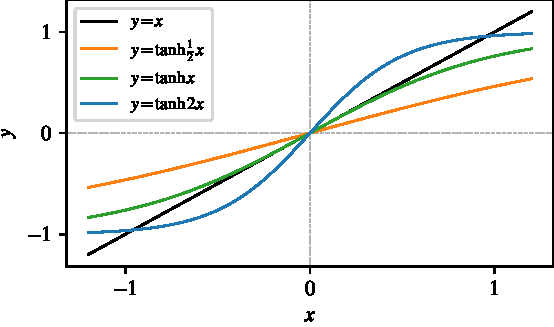
\includegraphics[width=0.7\linewidth]{ch4/cw_tanh.pdf}
\caption[Graphical solution to Curie--Weiss self-consistent equation]{
Graphical solution to the Curie--Weiss self-consistent equation in \cref{eq:cw}, where $x = -m$. The equation $x = \tanh a x$ has non-zero solutions only when $a = 2 d \beta (-J) > 1$.
}
\label{fig:cw-tanh}
\end{figure}

The non-interacting Hamiltonian \cref{eq:ham-mf-noninter} also implies that the joint probability $p(\vs)$ can be factorized into univariate probabilities:
\begin{align}
p_\text{MF}(\vs) &= \prod_i p_{\text{MF}\,i}(s_i), \\
p_{\text{MF}\,i}(s_i) &= \frac{\rme^{-\beta H_{\text{MF}\,i}(s_i)}}{\sum_s \rme^{-\beta H_{\text{MF}\,i}(s)}}.
\end{align}
Simplifying $p_\text{MF}(s_i)$ with \cref{eq:cw}, we have
\begin{equation}
p_\spinup = p_{\text{MF}\,i}(s_i = +1) = \frac{1 + m}{2}, \quad
p_\spindown = p_{\text{MF}\,i}(s_i = -1) = \frac{1 - m}{2}.
\label{eq:p-mf}
\end{equation}
The probability distribution $p_\text{MF}(\vs)$ can serve as a variational ansatz with a single tunable parameter $m$, which we refer to as the naive mean-field (NMF) ansatz.

Next, we use the NMF ansatz and the original Hamiltonian in \cref{eq:cl-ising} to evaluate the variational energy. The energy can be directly evaluated by
\begin{align}
E_\text{MF} &= \sum_\vs p_\text{MF}(\vs) H(\vs) \\
&= N d J (p_\spinup p_\spinup - p_\spinup p_\spindown - p_\spindown p_\spinup + p_\spindown p_\spindown) \\
&= N d J m^2, \\
\shortintertext{and the entropy is}
S_\text{MF} &= -\sum_\vs p_\text{MF}(\vs) \ln p_\text{MF}(\vs) \\
&= -N (p_\spinup \ln p_\spinup + p_\spindown \ln p_\spindown).
\end{align}
Under this ansatz, the free energy $F_\text{MF} = E_\text{MF} - \frac{1}{\beta} S_\text{MF}$ is the same as \cref{eq:fe-mf} derived from the approximated Hamiltonian. It is indeed an upper bound of the true free energy, as it is now derived from the variational ansatz on the original Hamiltonian. For more complicated models on non-regular graphs and with more than two-body interactions, where a self-consistent equation like \cref{eq:cw} cannot be easily constructed, we can still apply the NMF ansatz to obtain a preliminary variational approximation.

\subsection{Bethe ansatz}
\label{sec:bethe}

Starting from an analytical solution to the 1D quantum Heisenberg model~\cite{bethe1931theorie}, the Bethe ansatz has become a gross term for methods to exactly solve or approximate partition functions on lattices and other graphs~\cite{baxter1995solvable, caravelli2022some, gujrati1995bethe, mezard2001bethe}. It is also deeply related to belief propagation, a message passing algorithm used in Bayesian inference and the recent trend of graph machine learning~\cite{yedidia2003understanding, ikeda2004stochastic}. Unlike the NMF ansatz which approximates the original model using only uniform global interactions, the Bethe ansatz utilizes the local geometry to more accurately represent interactions between nearest neighbors.

In general, the Bethe ansatz is applicable to any probability distribution defined on a graph $\calG = (\calV, \calE)$, where $\calV$ is the set of sites and $\calE$ is the set of edges, as long as the probability of each configuration can be factorized into two-body interactions:
\begin{equation}
p(\vs) = \frac{1}{Z} \prod_{(i, j) \in \calE} f_{i j}(s_i, s_j).
\end{equation}
For the Ising model in \cref{eq:cl-ising}, we have
\begin{equation}
f_{i j}(s_i, s_j) = \rme^{-\beta J s_i s_j}.
\end{equation}

To study the properties of an edge or a site while marginalizing the rest of the graph, we define the auxiliary probability with an edge $(i j)$ removed from the graph:
\begin{align}
\mu^{(i j)}(\vs) &= \frac{1}{Z^{(i j)}} \prod_{(k, l) \in \calE \setminus (i j)} f_{k l}(s_k, s_l), \\
\shortintertext{and with all edges on the site $i$ removed from the graph:}
\mu^{(i)}(\vs) &= \frac{1}{Z^{(i)}} \prod_{(k, l) \in \calE, i \notin \{k, l\}} f_{k l}(s_k, s_l),
\end{align}
where $Z^{(i j)}$ and $Z^{(i)}$ are corresponding normalization constants. We also evaluate the marginal probabilities
\begin{align}
\mu^{(i j)}_i(s_i) &= \sum_{\vs_{\calV \setminus i}} \mu^{(i j)}(s_i, \vs_{\calV \setminus i}), \\
\mu^{(i j)}_{i j}(s_i, s_j) &= \sum_{\vs_{\calV \setminus \{i, j\}}} \mu^{(i j)}(s_i, s_j, \vs_{\calV \setminus \{i, j\}}), \\
\mu^{(i)}_{\partial i}(\vs_{\partial i}) &= \sum_{\vs_{\calV \setminus \partial i}} \mu^{(i)}(\vs_{\partial i}, \vs_{\calV \setminus \partial i}),
\end{align}
where $\partial i = \left\{ j \mid (i, j) \in \calE \right\}$ denotes the neighbors of the site $i$. The univariate marginal probability with an edge removed is denoted by the ``message'':
\begin{equation}
\mu_{i \to j}(s_i) = \mu^{(i j)}_i(s_i).
\end{equation}
After removing the edge $(i, j)$, there is no interaction between $i$ and $j$ after marginalizing other sites, so we have
\begin{equation}
\mu^{(i j)}_{i j}(s_i, s_j) = \mu_{i \to j}(s_i) \mu_{j \to i}(s_j).
\end{equation}

Then we write down the relation between $\mu^{(i j)}(\vs)$ and $\mu^{(i)}(\vs)$. Temporarily ignoring the normalization constants, we can marginalize $\mu^{(i j)}(\vs)$ by first marginalizing $\mu^{(i)}(\vs)$ and then evaluating the remaining interactions between $i$ and $\partial i \setminus j$:
\begin{equation}
\mu^{(i j)}_{i j}(s_i, s_j) \propto \sum_{\vs_{\partial i \setminus j}} \mu^{(i)}_{\partial i}(s_j, \vs_{\partial i \setminus j}) \prod_{k \in \partial i \setminus j} f_{i k}(s_i, s_k).
\end{equation}
It is proposed to approximate the environment to the site $i$ by the product of messages:
\begin{equation}
\mu^{(i)}_{\partial i}(\vs_{\partial i}) \approx \prod_{j \in \partial i} \mu_{j \to i}(s_j).
\label{eq:bethe-prob}
\end{equation}
Now we have the self-consistent equations
\begin{align}
\mu_{i \to j}(s_i) &\propto \sum_{\vs_{\partial i \setminus j}} \prod_{k \in \partial i \setminus j} \mu_{k \to i}(s_k) \prod_{k \in \partial i \setminus j} f_{i k}(s_i, s_k) \\
&= \prod_{k \in \partial i \setminus j} \sum_{s_k} f_{i k}(s_i, s_k) \mu_{k \to i}(s_k),
\label{eq:bethe-message}
\end{align}
from which we can solve the $4 N d$ variables $\mu_{i \to j}(s_i)$. After recovering the normalization constants in \cref{eq:bethe-message}, they can be solved by iterative algorithms if the convergence conditions are satisfied~\cite{mooij2007sufficient}, or by gradient-based algorithms.

Given the messages, we can obtain the two-body marginals of the original distribution
\begin{equation}
\mu_{i j}(s_i, s_j) = \frac{f_{i j}(s_i, s_j) \mu_{i \to j}(s_i) \mu_{j \to i}(s_j)}{\sum_{s'_i, s'_j} f_{i j}(s'_i, s'_j) \mu_{i \to j}(s'_i) \mu_{j \to i}(s'_j)},
\end{equation}
and estimate the energy and other observables with at most two-body interactions. For the Ising model in \cref{eq:cl-ising}, we have
\begin{equation}
E_\text{Bethe} = J \sum_{\langle i, j \rangle} \mu_{i j}(s_i, s_j) s_i s_j.
\end{equation}
We can also construct a Bethe entropy from the edge terms and the site terms:
\begin{align}
S_\text{Bethe} &= S_\calE + S_\calV, \\
S_\calE &= -\sum_{(i, j) \in \calE} \ln \sum_{s_i, s_j} f_{i j}(s_i, s_j) \mu_{i \to j}(s_i) \mu_{j \to i}(s_j), \\
S_\calV &= \sum_i \ln \sum_{s_i} \prod_{j \in \partial i} \sum_{s_j} f_{i j}(s_i, s_j) \mu_{j \to i}(s_j),
\end{align}
and the Bethe free energy $F_\text{Bethe} = E_\text{Bethe} - \frac{1}{\beta} S_\text{Bethe}$.

When the graph is a tree, including a 1D chain, there actually exists a probability distribution $p_\text{Bethe}(\vs)$ that produces the marginals $\mu_{i j}(s_i, s_j)$ and the energy $E_\text{Bethe}$, and its entropy is exactly $S_\text{Bethe}$, so the Bethe ansatz can serve as a variational ansatz. However, for general graphs, $S_\text{Bethe}$ no longer equals the entropy of $p_\text{Bethe}(\vs)$, so $F_\text{Bethe}$ is not guaranteed to be an upper bound of the true free energy. Nevertheless, it is a close approximation in many cases. Similar techniques have been generalized to systems beyond two-body interactions, known as cluster variation methods~\cite{pelizzola2005cluster}.

\section{Neural network ansatzes}
\label{sec:nn}

\subsection{Layers in neural networks}

As introduced in \cref{sec:intro-ml}, neural networks in modern machine learning are composed of a common set of simple functions, known as ``layers'', and the composition can be arbitrarily sophisticated. The basic architecture among them is the feedforward neural network (FFNN), which is defined by a sequential composition of alternating linear layers and nonlinear activation layers:
\begin{equation}
\vy = (\text{Lin}_1 \circ \text{Act}_1 \circ \text{Lin}_2 \circ \text{Act}_2 \circ \cdots \circ \text{Lin}_{n_\text{l}} \circ \text{Act}_{n_\text{l}})(\vx),
\label{eq:ffnn}
\end{equation}
where $\vx$ is the inputs to the network, $\vy$ is the outputs, $n_\text{l}$ is the number of layers, and $\circ$ denotes function composition. This architecture is sketched in \cref{fig:nn-arch}.

\begin{figure}[htb]
\centering
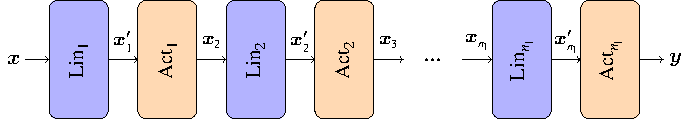
\includegraphics[width=0.9\linewidth]{ch4/nn_arch.pdf}
\caption[Architecture of feedforward neural network (FFNN)]{
Architecture of FFNN, which is a sequential composition of alternating linear layers Lin$_i$ and nonlinear activation layers Act$_i$. Each layer contains its own parameters. The values $\vx_i$ and $\vx'_i$ are outputs from the previous layer, which become inputs to the next layer.
}
\label{fig:nn-arch}
\end{figure}

The linear\footnote{It is technically an affine transformation rather than a linear transformation of $\vx_i$, because $\vb_i$ is included, but the name ``linear layer'' is commonly used in neural networks.} layer is defined by
\begin{equation}
\text{Lin}_i(\vx_i) = \mW_i \vx_i + \vb_i,
\label{eq:linear-layer}
\end{equation}
where $\mW_i$ is called the weight and $\vb_i$ the bias, which are the parameters of this layer. At this point, the parameters are not shared between layers. Assuming $\vx_i$ is a vector of size $n_{\text{in}\,i}$, we can choose an output size $n_{\text{out}\,i}$, then $\mW_i$ is inferred to be a matrix of size $n_{\text{out}\,i} \times n_{\text{in}\,i}$, $\vb_i$ is a vector of size $n_{\text{out}\,i}$, and the input size of the next linear layer $n_{\text{in}\,i + 1}$ equals $n_{\text{out}\,i}$.
In practice, the inputs $\vx_i$ have an additional batch dimension, which denotes the evaluation of the same network on different input samples, but it is omitted in our discussion for simplicity. The sizes of the intermediate outputs are known as the ``hidden sizes'', and the hyperparameters of the network include the number of layers and the hidden sizes. These hyperparameters, in contrast to the parameters $\mW_i$ and $\vb_i$, define the network architecture and mainly determine its expressiveness.

The activation layer, also known as the activation function, is an element-wise function of the input vector. A great variety of activation functions have been proposed, each with its own claimed advantages, but most are proven in practice to have only a minuscule impact on the expressiveness of the whole network, apart from the major difference in the output domain~\cite{kunc2024three}. The simplest choice is the rectified linear unit (ReLU):
\begin{equation}
\text{ReLU}(x) = \begin{cases}
x, & x > 0 \\
0, & x \le 0
\end{cases}.
\end{equation}
It has been used since the early research on neural networks, and is still efficient today despite its simplicity.

A modern choice is the Gaussian error linear unit (GELU)~\cite{hendrycks2016gaussian}:
\begin{equation}
\text{GELU}(x) = x\,\Phi(x),
\end{equation}
where $\Phi(x)$ is the cumulative distribution function (CDF) of the unit Gaussian distribution. While having the same asymptotic behaviors at $x \to \pm \infty$ as ReLU, it is derived from the stochastic regularization of the network and helps to stabilize the evaluation and the training of the network. It is the default choice in the NetKet software package~\cite{carleo2019netket}, and is used in most of the results reported in this thesis.

In particular, the activation function in the last layer can be the identity function if the outputs are unconstrained in $\bbR$, or specifically constructed to constrain the outputs in an interval. In the latter case, a common choice is the sigmoid function:
\begin{equation}
\text{Sigmoid}(x) = \frac{1}{1 + \rme^{-x}},
\label{eq:sigmoid}
\end{equation}
which maps from $\bbR$ to $(0, 1)$, or to another interval with an additional linear transform. The shapes of ReLU, GELU, and sigmoid are shown in \cref{fig:activations}.

\begin{figure}[htb]
\centering
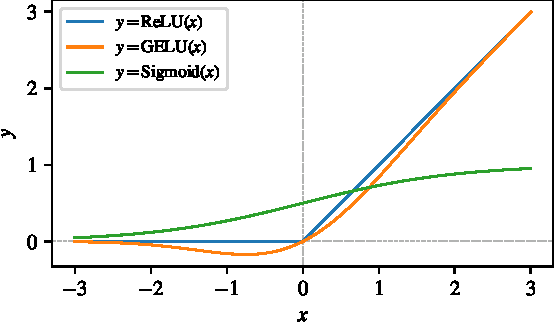
\includegraphics[width=0.7\linewidth]{ch4/nn_activations.pdf}
\caption[Commonly used activation functions in neural networks]{
Commonly used activation functions ReLU, GELU, and sigmoid in neural networks.
Both ReLU and GELU have asymptotic behaviors $y \to 0$ when $x \to -\infty$ and $y \to x$ when $x \to +\infty$, while GELU has more subtle nonlinearity around $x = 0$.
In contrast, the output of sigmoid is bounded in $(0, 1)$.
}
\label{fig:activations}
\end{figure}

\subsection{Symmetries in neural networks: convolutional and pooling layers}

Many-body systems usually have symmetries and locality, which also arise in machine learning of natural images. To take these advantages, the linear layers can be specialized into convolutional layers. Ignoring the layer index, a convolutional layer is denoted by $\vy = \text{Conv}(\vx)$, and in the 1D case it is defined by
\begin{equation}
y_{i, c} = \left( \sum_{k = 1}^{n_\text{k}} \sum_{c' = 1}^{n_\text{c in}} W_{k, c, c'} x_{i + k - 1, c'} \right) + b_{i, c},
\label{eq:conv-layer}
\end{equation}
where $\vx$ is an array of size $n_\text{s} \times n_\text{c in}$, $\vy$ is an array of size $n_\text{s} \times n_\text{c out}$, and we assume that the spatial dimension $n_\text{s}$ is the same in the inputs and the outputs for simplicity. Both the inputs and the outputs have another dimension of ``channels'', also known as ``features'', which determines the size of the network. The convolutional layer acts as if it were a linear layer on the channel dimension, mapping from $n_\text{c in}$ channels to $n_\text{c out}$ channels. It performs a convolution only on the spatial dimension, rather than on the channel dimension. The weights $\mW$ are an array of size $n_\text{k} \times n_\text{c out} \times n_\text{c in}$, where $n_\text{k}$ is the convolution kernel size, and the biases $\vb$ are an array of size $n_\text{k} \times n_\text{c out}$. Higher-dimensional convolutional layers can be defined similarly. In contrast to the convolutional layer, the general linear layer is also known as the dense layer. The FFNN with convolutional layers is known as the convolutional neural network (CNN).

In \cref{eq:conv-layer}, care should be taken when accessing the out-of-boundary values $x_{i, c}$ where $i > n_\text{s}$. For physical systems with open boundary conditions, the common practice is to pad with zeros: $x_{i, c} = 0$~\cite{islam2020much}; while for periodic boundary conditions, the convolution can be correspondingly periodic: $x_{i, c} = x_{i - n_\text{s}, c}$. In the latter case, the convolutional layer is translational equivariant in the spatial dimension, which means a translation of the inputs leads to the same translation of the outputs:
\begin{equation}
f(T_d \vx) = T_d f(\vx),
\end{equation}
where $T_d$ denotes the translation by $d$ steps: $T_d (x_1, \ldots, x_{n_\text{s}})$ = $(x_{1 + d}, x_{2 + d}, \ldots, x_{n_\text{s}}, x_1, x_2, \ldots, x_d)$, and $f$ is a neural network composed of convolutional and activation layers. Beyond translational symmetry, this equivariance can be generalized to more symmetry groups, such as rotations and reflections~\cite{luo2021gauge, roth2021group}.

There is also a kind of special linear layers known as pooling layers, which are invariant under the symmetry operations:
\begin{equation}
f(T_d \vx) = f(\vx),
\label{eq:trans-invar}
\end{equation}
where $f$ is a neural network composed of convolutional, activation, and pooling layers. For the purpose of this thesis, we may use the sum pooling as the last linear layer, which sums over the vector input to obtain a scalar output:
\begin{equation}
\text{Pool}(\vx) = \sum_{i = 1}^{n_\text{s}} x_i.
\end{equation}

\subsection{Neural network as variational ansatz}

After introducing the various layers as building blocks, we proceed to apply a neural network as the ansatz for a many-body system of $N$ spins. One may naively define
\begin{align}
q_\theta(\vs) &= \frac{1}{Z} \text{NN}(\vs), \\
Z &= \sum_\vs \text{NN}(\vs),
\end{align}
where NN is a neural network with input size $N$ and a scalar output, and $\theta$ denotes all parameters in it. However, the normalization constant $Z$ is an intractable sum of exponentially many configurations, and this distribution is not easier to sample from than the Boltzmann distribution; therefore, it cannot be directly used for MCMC importance sampling in \cref{eq:mcmc-importance}, or for variational inference in \cref{eq:fq}.

Some early attempts have been proposed to choose a simple ansatz that allows efficient cluster updates, such as a two-body interacting Hamiltonian~\cite{liu2017self} or a restricted Boltzmann machine (RBM)~\cite{huang2017accelerated}, and use it in \cref{eq:mcmc-importance}. As the normalization constant of the ansatz is still intractable, and thus the variational inference is inapplicable, the parameters of the ansatz are trained in a supervised learning approach. One first generates some samples from the target distribution using traditional MCMC, and then optimizes the energies of these samples evaluated by the ansatz towards those evaluated by the original Hamiltonian. After training, more samples can be generated from the ansatz using efficient cluster updates. However, the quality of the samples used in the training limits the accuracy of this approach.

Another approach is to specifically construct a neural network with tractable normalized probability. A prominent family of such an approach is the autoregressive models, which we will discuss in \cref{ch:arnn}. Moreover, a notable family of neural networks with this property is the normalizing flows~\cite{song2017nice, muller2019neural}, which reparameterize the target distribution into a simple one using the same principle as \cref{eq:reparam}. They are mostly used for continuous variables, which are beyond the scope of this thesis.

In addition to neural networks, tensor networks~\cite{bridgeman2017hand} with chain or tree geometries also support tractable normalized probability, which we will discuss in \cref{ch:tn}. However, they are more naturally defined and frequently used as variational ansatzes in quantum systems, while in classical systems they are usually used to approximate the partition function as a generalization of the transfer matrix to higher dimensions~\cite{verstraete2006criticality, vanderstraeten2018residual, vanhecke2021solving, lanthier2024tensor}.

A lesser known family of machine learning models that share this property are the sum-product networks~\cite{poon2011sum}, which define complicated multivariate distributions using directed graphs. They have been applied to various fields of machine learning~\cite{sanchez2022sum}, and they receive renewed attention with the recently proposed Kolmogorov--Arnold networks (KANs)~\cite{liu2024kan}, but their usage is still not as prevalent as neural networks due to limited support in hardware and software~\cite{barham2019machine}.
